\section{Режимы работы блоковых шифров}
\selectlanguage{russian}

Открытый текст $M$, представленный как двоичный файл, перед шифрованием разбивают на части $M_1, M_2, \dots, M_n$, называемые пакетами. Предполагается, что размер в битах каждого пакета существенно превосходит длину блока шифрования, которая равна 64 бита для российского стандарта и 128 для американского стандарта AES.

В свою очередь, каждый пакет $M_i$ разбивается на блоки размера, равного размеру блока шифрования:
    \[ M_i = \left[ M_{i,1}, M_{i,2}, \dots, M_{i,n_i} \right]. \]
Число блоков $n_i$ в разных пакетах может быть разным. Кроме того, последний блок пакета $M_{i,n_i}$ может иметь размер, меньший размера блока шифрования. В этом случае для него применяют процедуру дополнения (удлинения) до стандартного размера. Процедура должна быть обратимой: после расшифрования последнего блока пакета лишние байты должны быть обнаружены и удалены. Некоторые способы дополнения:
\begin{itemize}
  \item добавить один байт со значением $128$, а остальные байты пусть будут нулевые;
  \item определить, сколько байтов надо добавить к последнему блоку, например $b$, и добавить $b$ байтов со значением $b$ в каждом.
\end{itemize}
В дальнейшем предполагается, что такое дополнение сделано для каждого пакета. При шифровании блоков внутри одного пакета первый индекс в нумерации блоков опускается, то есть вместо обозначения $M_{i,j}$ используется $M_j$.

Для шифрования всего открытого текста $M$ и, следовательно, всех пакетов используется один и тот же  \emph{сеансовый} ключ шифрования  $K$. Процедуру передачи одного пакета будем называть \emph{сеансом}.

Существует несколько режимов работы блоковых шифров: режим электронной кодовой книги, режим шифрования зацепленных блоков, режим обратной связи, режим шифрованной обратной связи, режим счетчика. Рассмотрим особенности каждого из этих режимов.


\subsection{Электронная кодовая книга}

В режиме электронной кодовой книги (аббревиатура ECB от английского названия Electronic Code Book) открытый текст в пакете разделен на блоки
    \[ \left[ M_1, M_2, \dots, M_{n-1}, M_n \right]. \]

В процессе шифрования каждому блоку $M_j$ соответствует свой шифротекст $C_j$, определяемый с помощью ключа $K$:
    \[ C_j = E_K(M_j), ~ j = 1, 2, \dots, n. \]

Если в открытом тексте есть одинаковые блоки, то в шифрованном тексте им также соответствуют одинаковые блоки. Это дает дополнительную информацию для криптоаналитика, что является недостатком этого режима. Другой недостаток состоит в том, что криптоаналитик может подслушивать, перехватывать, переставлять, воспроизводить ранее записанные блоки, нарушая конфиденциальность и целостность информации. Поэтому при работе в режиме электронной кодовой книги нужно вводить аутентификацию сообщений.

Шифрование в режиме электронной кодовой книги не использует сцепление блоков и синхропосылку\index{синхропосылка} (вектор инициализации)\index{вектор инициализации}. Поэтому для данного режима применима атака на различение сообщений, так как два одинаковых блока или два одинаковых открытых текста шифруются одинаково.

На рис. \ref{fig:ecb-demo} приведен пример шифрования графического файла морской звезды в формате BMP, 24 бита цветности на пиксел (рис. \ref{fig:starfish}), блоковым шифром AES с длиной ключа 128 бит в режиме электронной кодовой книги  (рис. \ref{fig:starfish-aes-128-ecb}). В начале зашифрованного файла был восстановлен стандартный заголовок формата BMP. Как видно, в зашифрованном файле изображение все равно различимо.
\begin{figure}[h!]
    \centering
    \subfloat[Исходный рисунок]{\label{fig:starfish} 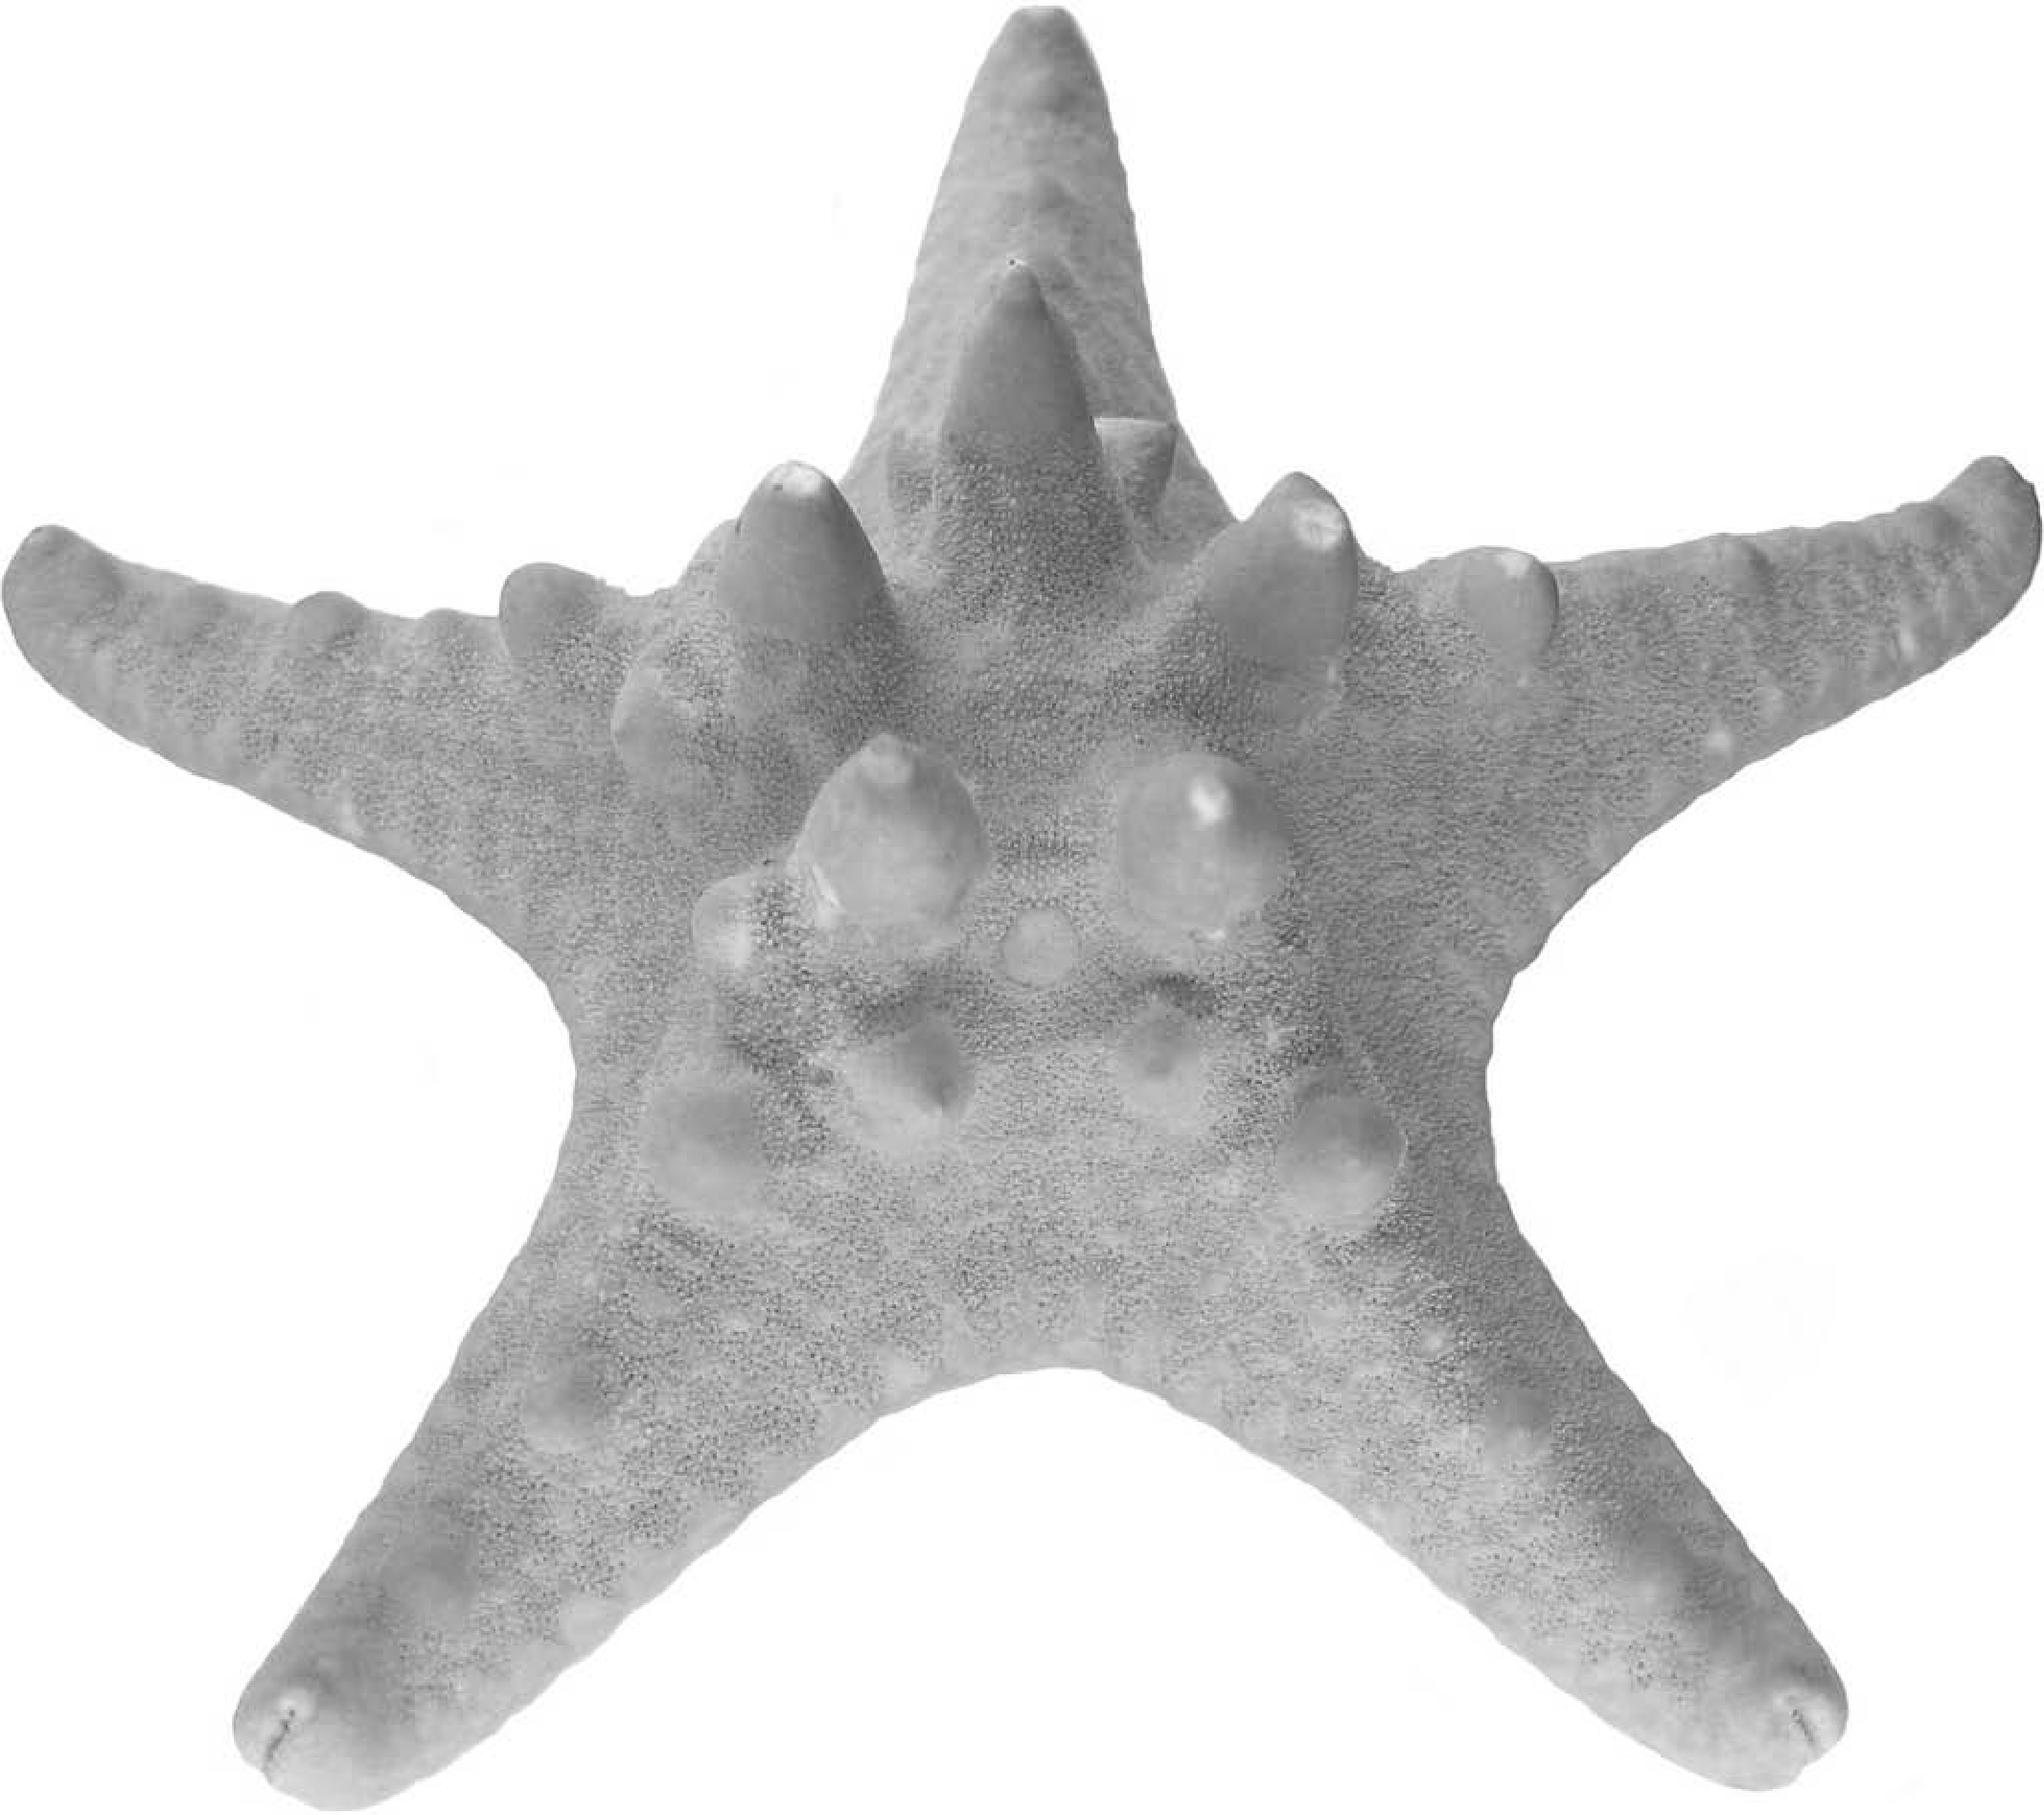
\includegraphics[width=0.45\textwidth]{pic/starfish}}
    ~~~
    \subfloat[Рисунок, зашифрованный AES-128]{\label{fig:starfish-aes-128-ecb} 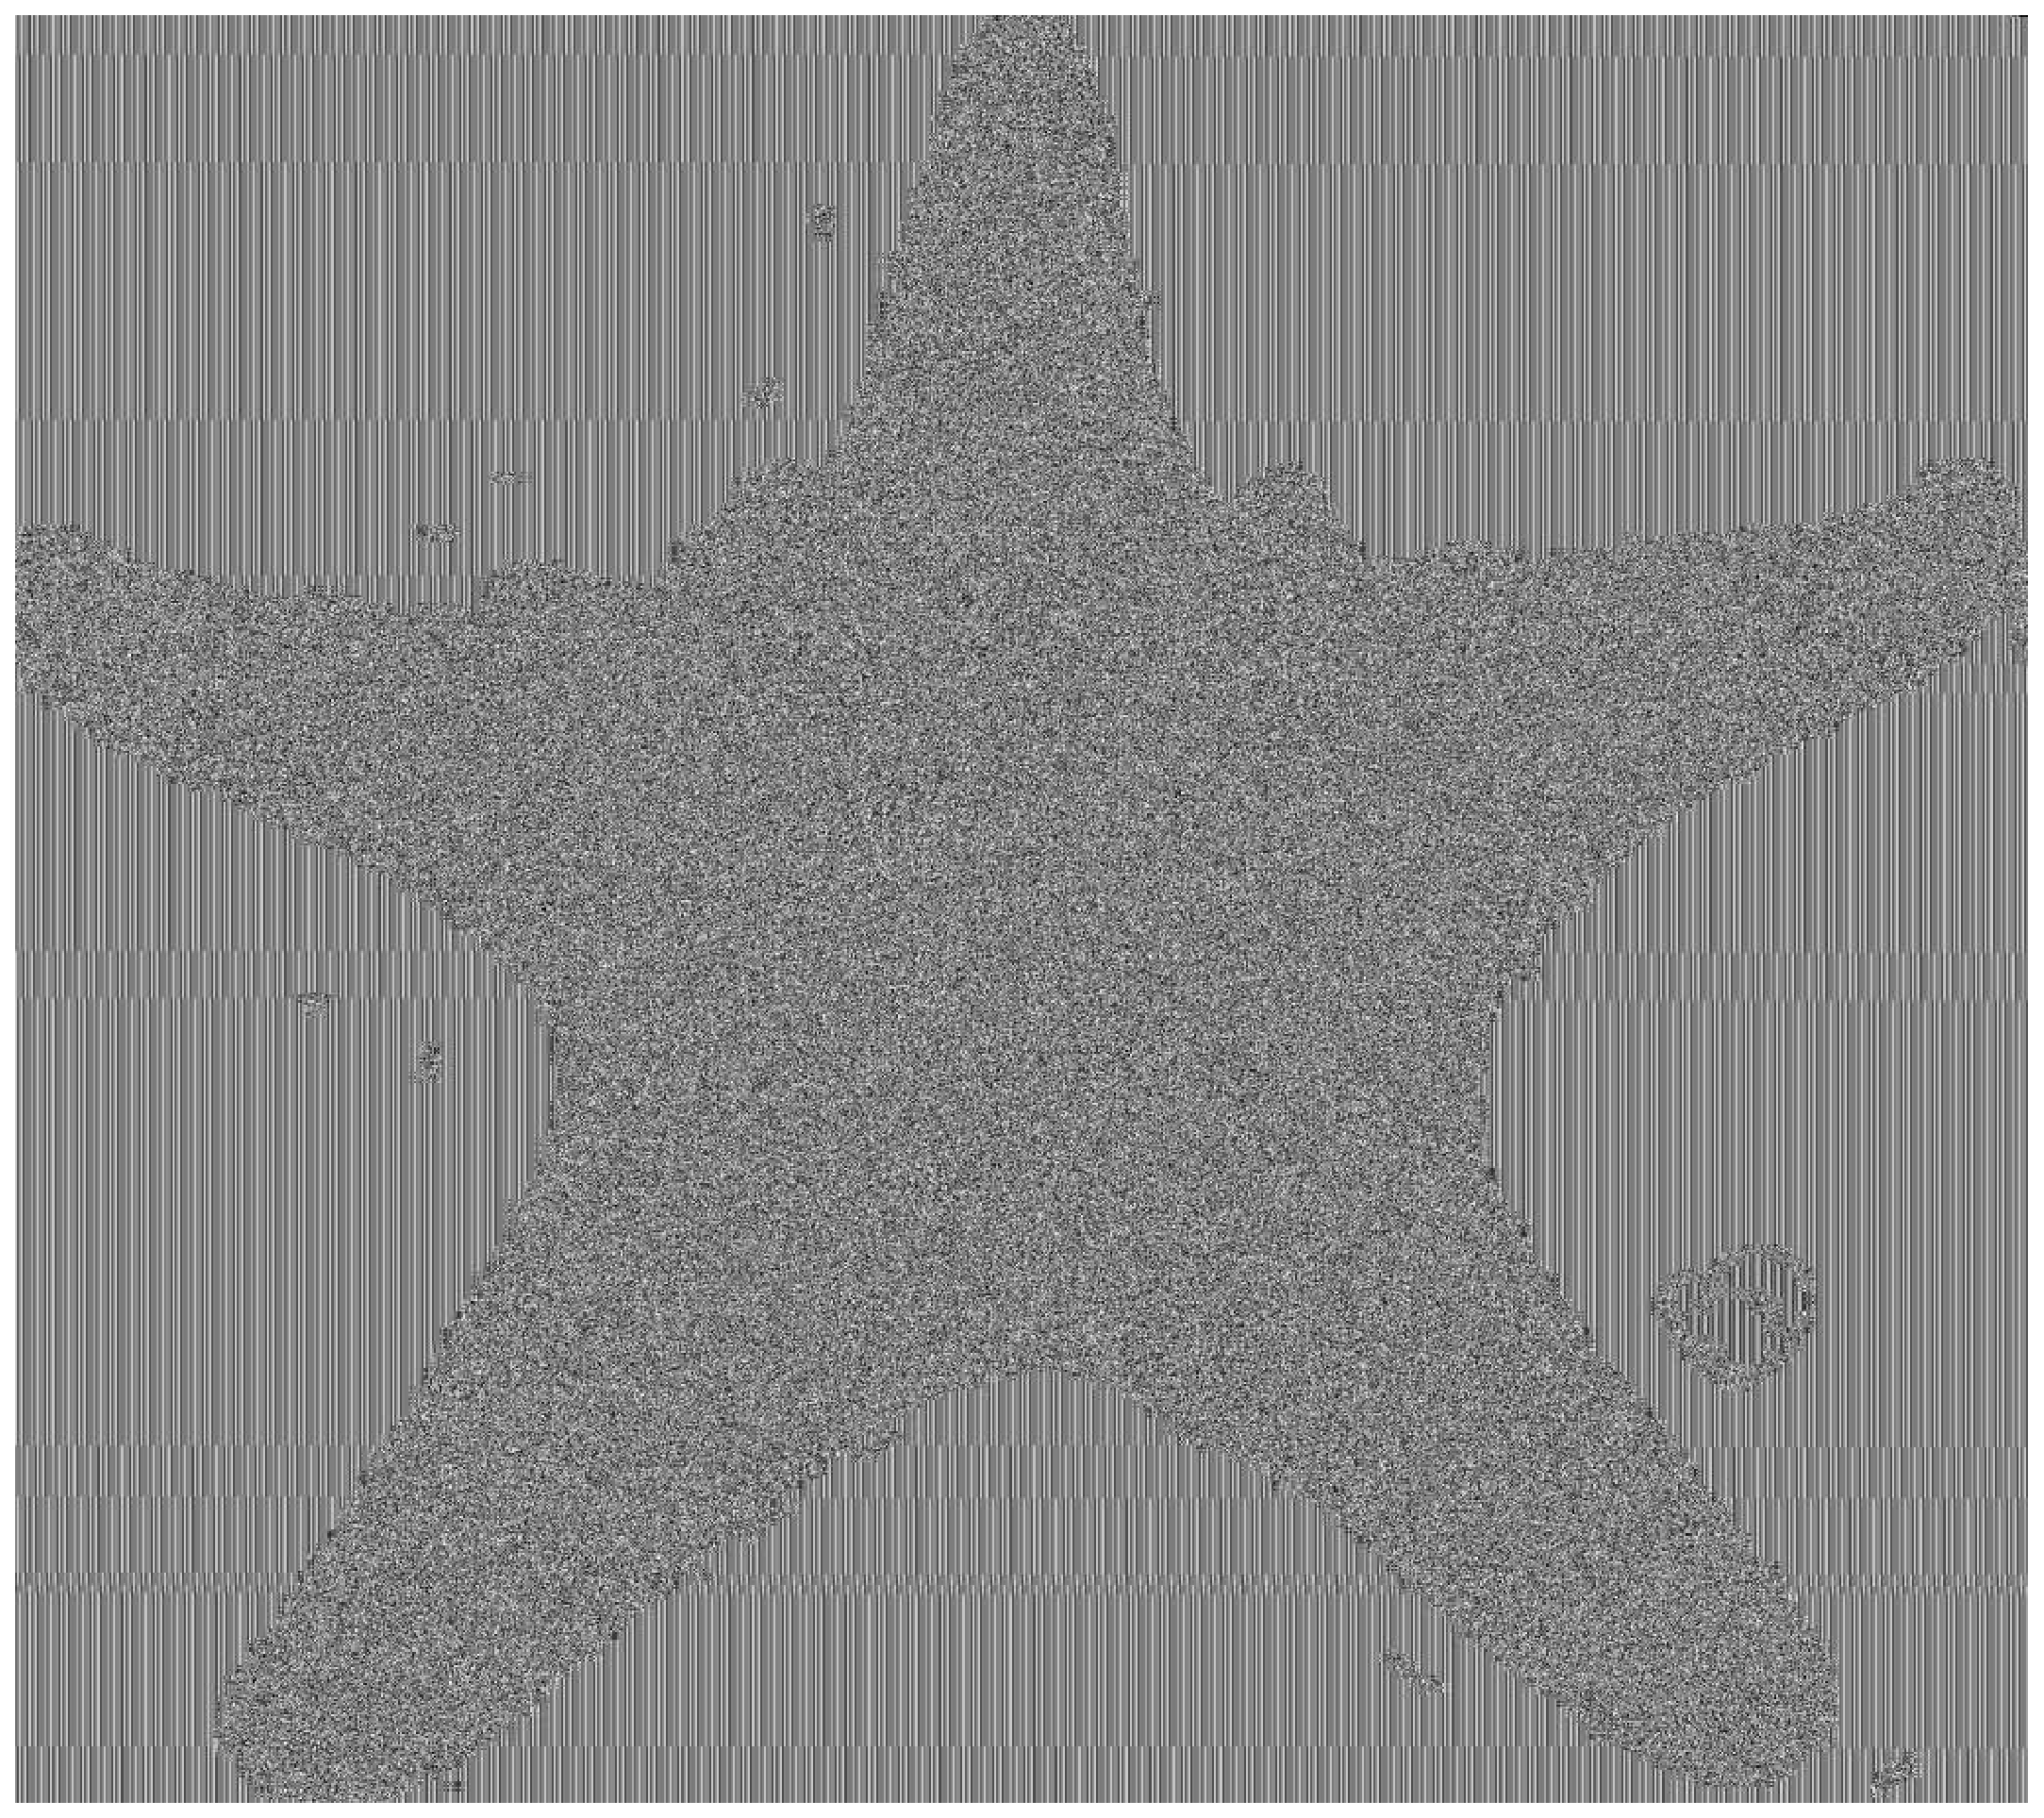
\includegraphics[width=0.45\textwidth]{pic/starfish-aes-128-ecb}}
    \caption{Шифрование в режиме электронной кодовой книги\label{fig:ecb-demo}}
\end{figure}
BMP файл в данном случае содержит в самом начале стандартный заголовок (ширина, высота, количество цветов) и далее идет массив 24-битовых значений цвета пикселов, взятых построчно сверху вниз. В массиве много последовательностей нулевых байтов, так как пикселы белого фона кодируются 3 нулевыми байтами. В AES размер блока равен 16 байтов и, значит, каждые $\frac{16}{3}$ подряд идущих пикселов белого фона шифруются одинаково, позволяя различить изображение в зашифрованном файле.

%На рис. \ref{fig:ecb-demo} приведен пример шифрования графического файла логотипа Википедии в формате BMP, 24 бита цветности на пиксел (рис. \ref{fig:wikilogo}), блоковым шифром AES с длиной ключа 128 бит в режиме электронной кодовой книги  (рис. \ref{fig:wikilogo-aes-128-ecb}). В начале зашифрованного файла был восстановлен стандартный заголовок BMP формата. Как видно, на зашифрованном рисунке возможно даже прочитать надпись.
%\begin{figure}[h!]
%    \centering
%    \subfloat[Исходный рисунок]{\label{fig:wikilogo}
\includegraphics[width=0.45\textwidth]{pic/wikilogo}}
%    ~~~
%    \subfloat[Рисунок, зашифрованный AES-128]{\label{fig:wikilogo-aes-128-ecb}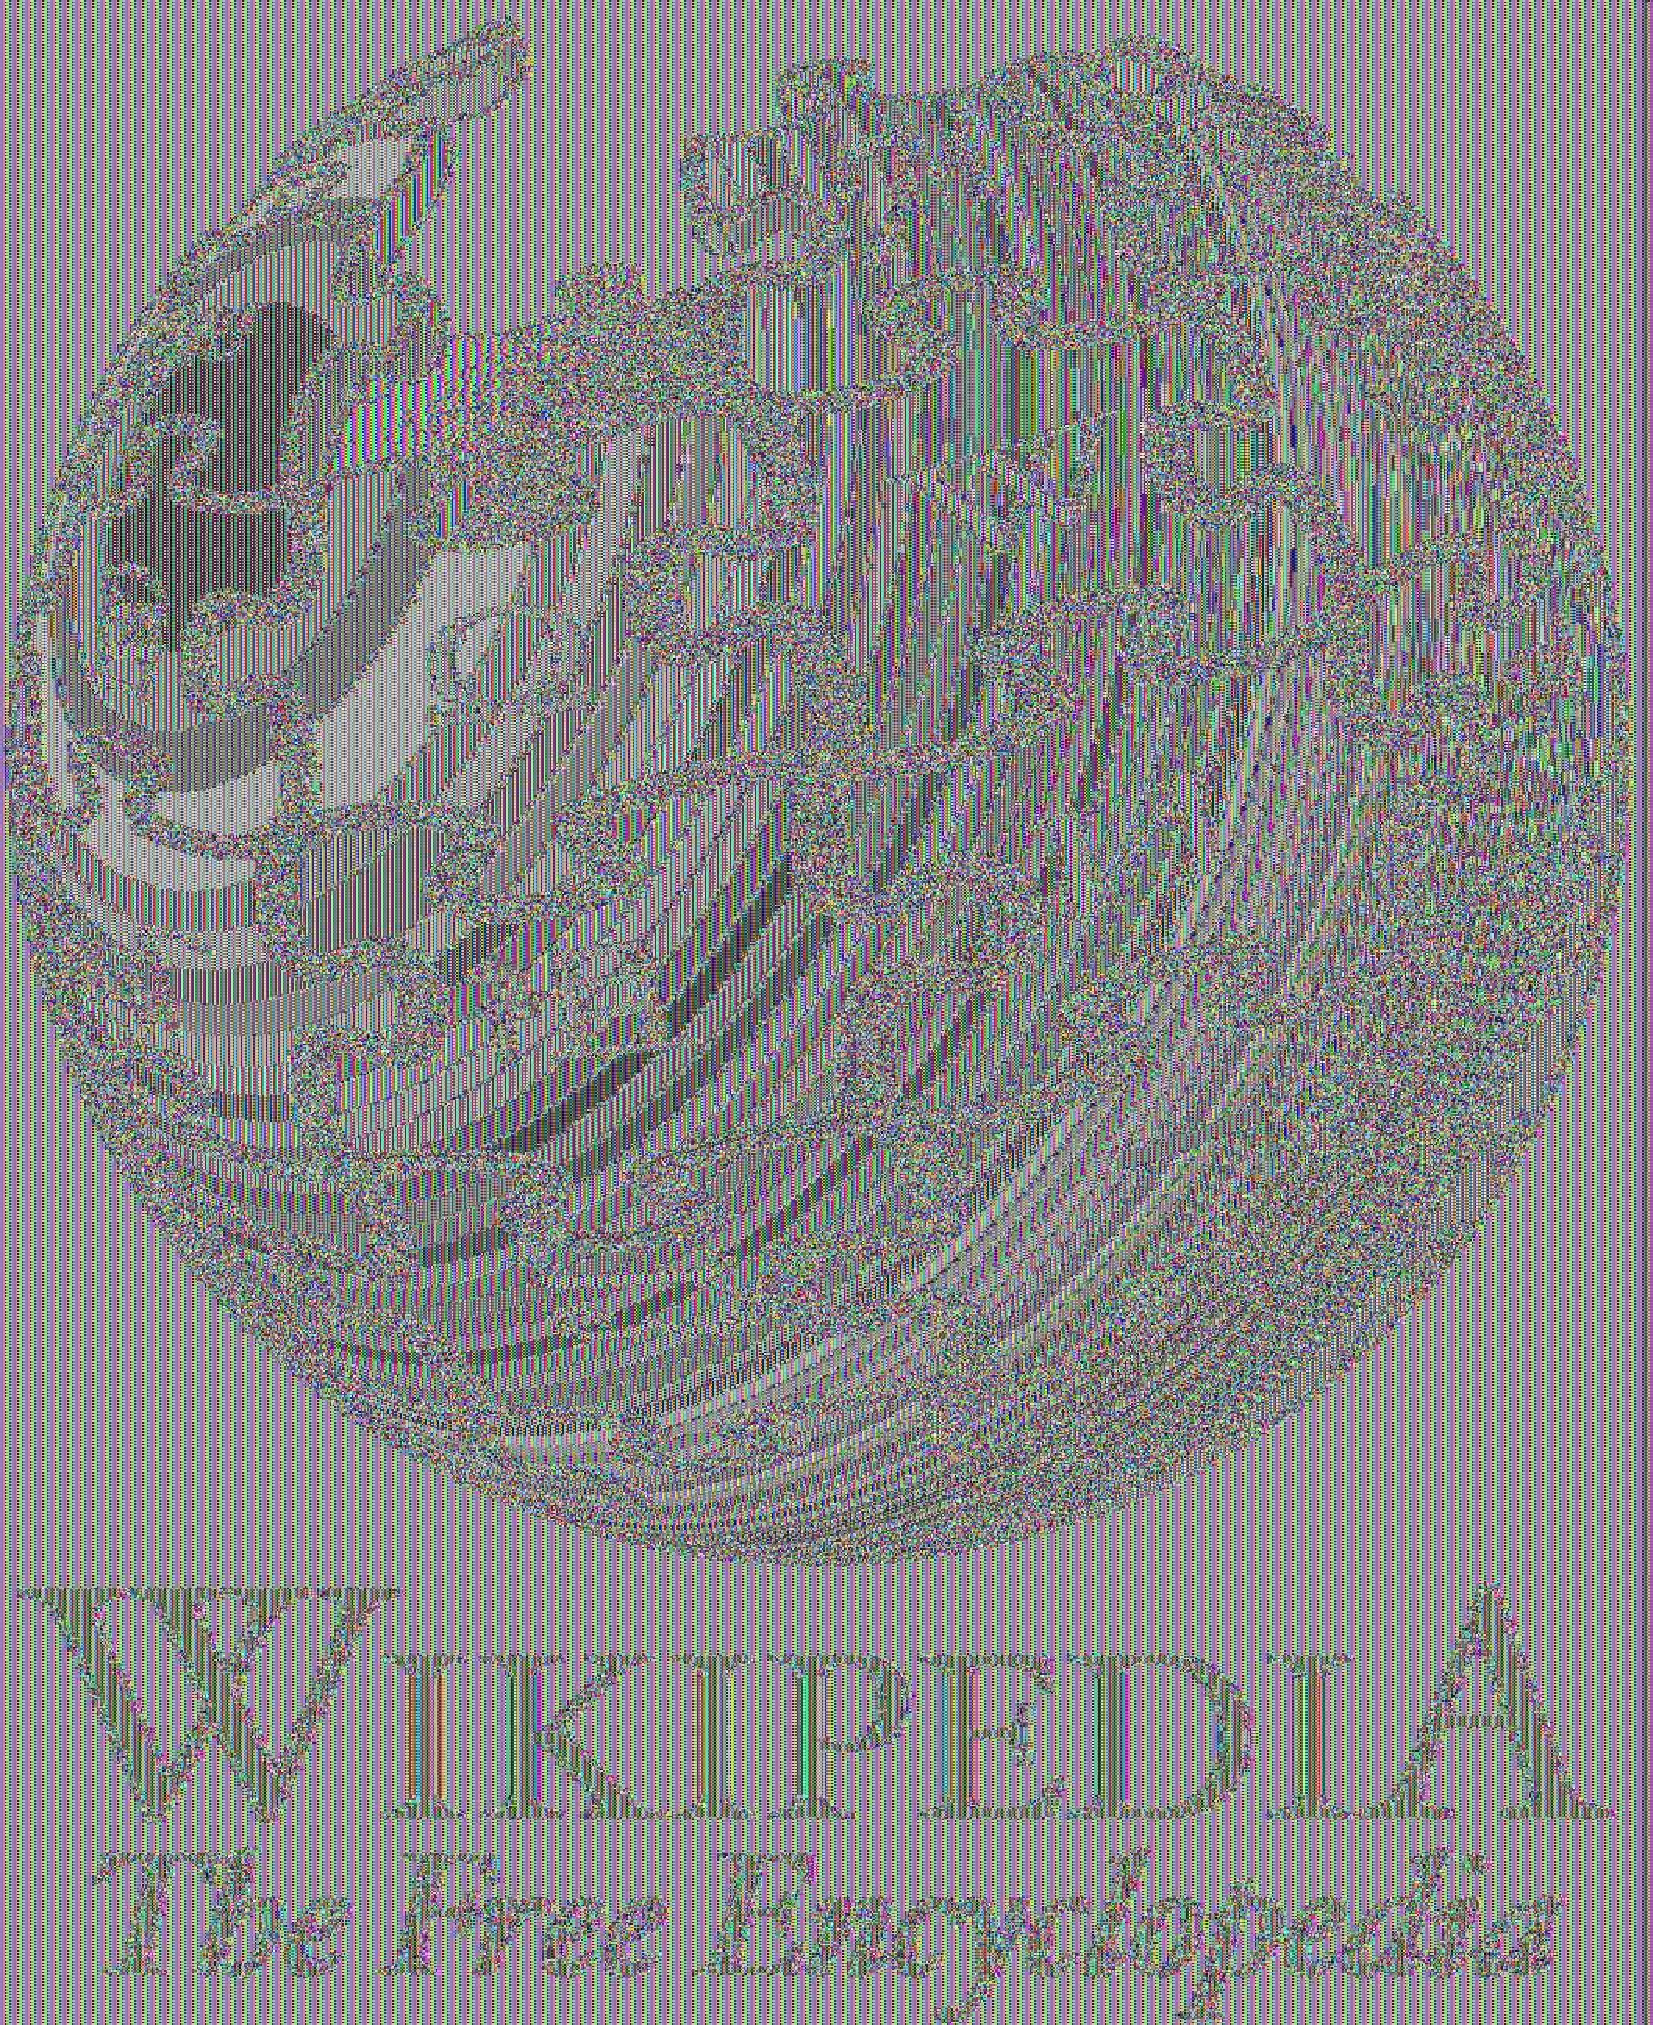
\includegraphics[width=0.45\textwidth]{pic/wikilogo-aes-128-ecb}}
%    \caption{Шифрование в режиме электронной кодовой книги.}
%    \label{fig:ecb-demo}
%\end{figure}

%Возможно воссоздание структуры информации -- например, пингвин на рис. \ref{fig:tux-ecbmode}. Картинка с пингвином записана в формате BMP и зашифрована DES в режиме электронной кодовой книги.
%\begin{figure}[h!]
%    \centering
%    \includegraphics[width=0.3\textwidth]{pic/tux-ecb}
%    \caption{Картинка с пингвином, зашифрованная в режиме электронной кодовой книги.}
%    \label{fig:tux-ecbmode}
%\end{figure}


\subsection{Сцепление блоков шифротекста}

В режиме сцепления блоков шифротекста (аббревиатура CBC от английского названия Cipher Block Chaining) перед шифрованием текущего блока открытого текста предварительно производится его суммирование по модулю 2 с предыдущим блоком зашифрованного текста, что и осуществляет <<сцепление>> блоков. Процедура шифрования имеет вид
\[ \begin{array}{l}
    C_1 = E_K(M_1 \oplus C_0), \\
    C_j = E_K(M_j \oplus C_{j-1}), ~ j = 1, 2, \dots,  n,
\end{array} \]
где $C_0 = \textrm{IV}$ --  вектор, называемый вектором инициализации (обозначение $\textrm{IV}$ от Initialization Vector). Другое название -- синхропосылка.

Благодаря сцеплению \emph{одинаковым} блокам открытого текста соответствуют \emph{различные} шифрованные блоки. Это затрудняет криптоаналитику статистический анализ потока шифрованных блоков.

На приемной стороне расшифрование осуществляется по правилу
\[ \begin{array}{l}
    D_K(C_j) = M_j \oplus C_{j-1}, ~ j=1, 2, \dots, n,\\
    M_{j} = D_K(C_j) \oplus C_{j-1}.
\end{array} \]

Блок $C_0 = \textrm{IV}$ должен быть известен легальному получателю шифрованных сообщений. Обычно криптограф выбирает его случайно и вставляет на первое место в поток шифрованных блоков. Сначала передают блок $C_0$, а затем шифрованные блоки $C_1, C_2, \ldots, C_n$.

В разных пакетах блоки $C_0$ должны выбираться независимо. Если их выбрать одинаковыми, то возникают проблемы, аналогичные проблемам в режиме ECB. Например, часто первые нешифрованные блоки $M_1$ в разных пакетах бывают одинаковыми. Тогда одинаковыми будут и первые шифрованные блоки.

Однако случайный выбор векторов инициализации также имеет свои недостатки. Для выбора такого вектора необходим хороший генератор случайных чисел. Кроме того, каждый пакет удлиняется на один блок.

Нужны такие процедуры выбора $C_0$ для каждого сеанса передачи пакета, которые известны криптографу и легальному пользователю. Одним из решений является использование так называемых \emph{одноразовых меток}. Каждому сеансу присваивается уникальное число. Его уникальность состоит в том, что оно используется только один раз и никогда не должно повторяться в других пакетах. В англоязычной научной литературе оно обозначается как \emph{Nonce}, то есть сокращение от <<Number used once>>\index{одноразовая метка}.

Обычно одноразовая метка состоит из номера сеанса и дополнительных данных, обеспечивающих уникальность. Например, при двустороннем обмене шифрованными сообщениями одноразовая метка может состоять из номера сеанса и индикатора направления передачи. Размер одноразовой метки должен быть равен размеру шифруемого блока. После определения одноразовой метки $\textrm{Nonce}$ вектор инициализации вычисляется в виде
    \[ C_0 = \textrm{IV} = E_K(\textrm{Nonce}). \]

Этот вектор используется в данном сеансе для шифрования открытого текста в режиме CBC. Заметим, что блок $C_0$ передавать в сеансе не обязательно, если приемная сторона знает заранее дополнительные данные для одноразовой метки. Вместо этого достаточно вначале передать только номер сеанса в открытом виде. Приемная сторона добавляет к нему дополнительные данные и вычисляет блок $C_0$, необходимый для расшифрования в режиме CBC. Это позволяет сократить издержки, связанные с удлинением пакета. Например, для шифра AES длина блока $C_0$ равна $16$ байтов. Если число сеансов ограничить величиной $2^{32}$ (вполне приемлемой для большинства приложений), то для передачи номера пакета понадобится только $4$ байта.


\subsection{Обратная связь по выходу}

В предыдущих режимах входными блоками для устройств шифрования были непосредственно блоки открытого текста.
В режиме обратной связи по выходу (OFB от Output FeedBack) блоки открытого текста непосредственно на вход устройства шифрования не поступают. Вместо этого устройство шифрования генерирует псевдослучайный поток байтов, который суммируется по модулю $2$ с открытым текстом для получения шифрованного текста. Шифрование осуществляют по правилу
\[ \begin{array}{l}
    K_0 = \textrm{IV}, \\
    K_j = E_K(K_{j-1}), ~ j = 1, 2, \dots, n, \\
    C_j = K_j \oplus M_j.
\end{array} \]

Здесь текущий ключ $K_j$ есть результат шифрования предыдущего ключа $K_{j-1}$. Начальное значение $K_0$ известно криптографу и легальному пользователю. На приемной стороне расшифрование выполняют по правилу
\[ \begin{array}{l}
    K_0 = \textrm{IV}, \\
    K_j = E_K(K_{j-1}), ~ j = 1, 2, \dots, n, \\
    M_j = K_j \oplus C_j.
\end{array} \]

Как и в режиме CBC, вектор инициализации $\textrm{IV}$ может быть выбран случайно и передан вместе с шифрованным текстом либо вычислен на основе одноразовых меток. Здесь особенно важна уникальность вектора инициализации.

Достоинство этого режима состоит в полном совпадении операций шифрования и расшифрования. Кроме того, в этом режиме не надо проводить операцию дополнения открытого текста.


\subsection{Обратная связь по шифрованному тексту}

В режиме обратной связи по шифрованному тексту (CFB от Cipher FeedBack) ключ $K_j$ получается с помощью процедуры шифрования предыдущего шифрованного блока $C_{j-1}$. Может быть использован не весь блок $C_{j-1}$, а только часть его. Как и в предыдущем случае, начальное значение ключа $K_0$ известно криптографу и легальному пользователю:
\[ \begin{array}{l}
    K_0 = \textrm{IV}, \\
    K_j = E_K(C_{j-1}), ~ j = 1, 2, \dots, n,\\
    C_j = K_j \oplus M_j.
\end{array} \]

У этого режима нет особых преимуществ по сравнению с другими режимами.


\subsection{Счетчик}

В режиме счетчика (CTR от Counter) правило шифрования имеет вид, похожий на режим обратной связи по выходу (OFB), но позволяющий вести независимое (параллельное) шифрование и расшифрование блоков:
\[ \begin{array}{l}
    K_j = E_K(\textrm{Nonce} \| j - 1), ~ j = 1, 2, \dots, n, \\
    C_j = M_j \oplus K_j,
\end{array} \]
где $\textrm{Nonce} \| j - 1$ -- конкатенация битовой строки одноразовой метки $\textrm{Nonce}$ и номера блока уменьшенного на единицу $j-1$.
%Для стандарта AES значение $\textrm{Nonce}$ занимает 16 бит, номер блока -- 48 бит. С одним ключом выполняется шифрование $2^{48}$ блоков.

Правило расшифрования идентичное:
\[ \begin{array}{l}
    M_j = C_j \oplus K_j. \\
\end{array} \]
